\documentclass[border=10pt]{standalone}
\usepackage{tikz}
\usetikzlibrary{arrows.meta}
\tikzset{%
  >={Latex[width=2mm,length=2mm]},
  % Specifications for style of nodes:
            base/.style = {rectangle, rounded corners, draw=black,
                           minimum width=4cm, minimum height=1cm,
                           text centered, font=\sffamily},
  activityStarts/.style = {base, fill=blue!30},
       startstop/.style = {base, fill=red!30},
    scoreDiff/.style = {base, fill=green!30},
         process/.style = {base, minimum width=2.5cm, fill=orange!15,
                           font=\ttfamily},
}
\begin{document}    
% Drawing part, node distance is 1.5 cm and every node
% is prefilled with white background
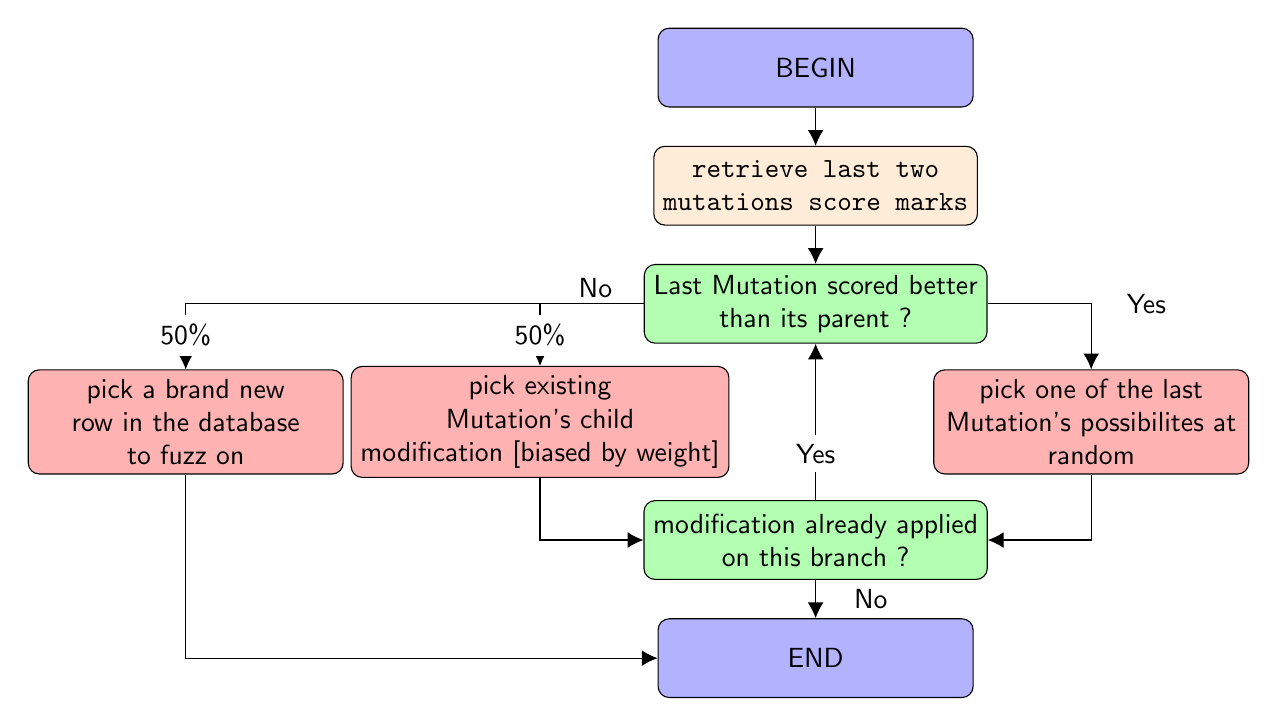
\begin{tikzpicture}[node distance=1.5cm,
    every node/.style={fill=white, font=\sffamily}, align=center]
  % Specification of nodes (position, etc.)
  \node (start) [activityStarts] {BEGIN};
  \node (retriveLastMutationsBlock)  [process, below of=start]  {retrieve last two \\ mutations score marks};
  \node (scoreDiff) [scoreDiff, below of=retriveLastMutationsBlock] {Last Mutation scored better \\ than its parent ?};
  \node (pickLastMutationChildBlock) [startstop, right of=scoreDiff, below of=scoreDiff, xshift=2cm] {pick one of the last \\ Mutation's possibilites at \\ random};
  \node (modifPerformedBlock) [scoreDiff, below of=scoreDiff, yshift=-1.5cm] {modification already applied \\ on this branch ?};
  \node (pickExistingBlock) [startstop, left of=scoreDiff, below of=scoreDiff, xshift=-2cm] {pick existing  \\ Mutation's child  \\ modification [biased by weight]};
  \node (pickNewRowBlock) [startstop, left of=pickExistingBlock,  xshift=-3cm] {pick a brand new \\ row in the database  \\ to fuzz on};
  \node (end) [activityStarts, below of=modifPerformedBlock] {END};     
  % Specification of lines between nodes specified above
  % with aditional nodes for description 
  \draw[->]     (start) 	-- (retriveLastMutationsBlock);
  \draw[->]     (retriveLastMutationsBlock) -- (scoreDiff);
  \draw[->]     (scoreDiff)	 -| node[yshift=0.2cm,xshift=20]{No} node[yshift=-0.4cm]{50\%} (pickExistingBlock);
  \draw[->]     (scoreDiff)	 -| node[yshift=-0.4cm]{50\%}(pickNewRowBlock);
  \draw[->]     (scoreDiff)  -| node[xshift=0.7cm]{Yes} (pickLastMutationChildBlock);
  \draw[->]    	(pickNewRowBlock)	 |- (end);
  \draw[->]    	(pickExistingBlock)	 |- (modifPerformedBlock);
  \draw[->]    	(pickLastMutationChildBlock)	 |-	 (modifPerformedBlock);
  \draw[->]    	(modifPerformedBlock)	 -- node[yshift=-0.4cm]{Yes}(scoreDiff);
  \draw[->]    	(modifPerformedBlock)	 -- node[xshift=0.7cm]{No} (end);
  \end{tikzpicture}
\end{document}